\documentclass[accentcolor=tud9c,colorbacktitle,inverttitle,landscape,german,presentation,t]{tudbeamer}
\usepackage{amstext}
\usepackage{amsmath}
\usepackage{graphicx}
\usepackage{multicol}
\usepackage{mathtools}
\usepackage{subfigure}
\usepackage[ngerman,english]{babel}
\usepackage[utf8]{inputenc}
\usepackage{colortbl}
\usepackage{adjustbox}

\begin{document}

\title{\"Ubung 7 - Gruppe 142}
\subtitle{Visual Computing - Grafikpipeline \& Eingabemodalit\"aten \& VR+AR} 

\author[Johannes Beck, Christian Eilers, Robin Menzenbach, Martin Steinborn]{Johannes Beck, Christian Eilers, Robin Menzenbach, Martin Steinborn}


\date{\today}

\begin{titleframe}
\end{titleframe}

\section{Aufgabe 1}
	\begin{frame}
		\frametitle{Aufgabe 1: Allgemeine Fragen}
		\begin{itemize}
		\item[a)]In der Augmented Reality soll die Wahrnehmung des Nutzers verbessert und vergrößert werden. So werden hier zusätzliche Informationen bereitgestellt, wie die Geschwindigkeit in einem Head-up Display oder anstehende Termine am Rand des Sichtfeldes.\\
In der Virtual Reality ist die virtuelle Welt das Ziel des Nutzers. Er möchte damit interagieren, und wenn möglich sollte er nicht bemerken sich in einer virtuellen Welt zu befinden.
		\item[b)]In der Computer Vision geht es darum, gegenstände in Bilder zu erkennen, in der Computergrafik möchte man gegenstände erzeugen. Im Endeffekt kann vision als umgekehrte Grafik betrachtet werden.
		\item[c)] 3D Objekte werden am Computer durch Polygon Netze mit Material, Beleuchtung in verschiedenen Szenen dargestellt.
		\end{itemize}
	\end{frame}


	\begin{frame}
		\frametitle{Aufgabe 1: Allgemeine Fragen}
		\begin{itemize}
		\item[d)]
		\begin{itemize}
			 \item[-] \textbf{Flat Shading}: Aufteilung in Primitive. Die orientierung normale des Primitives ergibt dann die Helligkeit.
			 \item[-] \textbf{Gouraud Shading}: Aufteilung in Primitive. Helligkeit wird über die Eckpunkte Normale berechnet und diese Werte entlang der Kanten des Primitives linear interpoliert.
			 \item[-] \textbf{Phong Shading}: Wie Gouraud Shading, nur wird die Helligkeit auch auf den Flächen der Primitive interpoliert.
		\end{itemize}
		\item[e)]  Hüllkörper umfassen Primitive, um Schnitt- oder Kollisionstests mit anderen Primitiven zu vereinfachen. Um dies zu gewährleisten, sollten Hüllkörper so einfach wie möglich aufgebaut sein, also Kugeln oder Bounding Boxes. Im 3-dimensionalen werden dann Kugeln oder Würfel verwendet.
		\end{itemize}
	\end{frame}

\section{Aufgabe 2}
	\begin{frame}
		\frametitle{Aufgabe 2: Geometrieverarbeitung}
		\begin{itemize}
		\item[a)] Zuerst wird das Sichtvolumen mithilfe der Model-Transformation an das Koordinatensystem angepasst. Danach werden die Texturen mit dem Painter's-Algorithmus gezeichnet. Dieser zeichnet die am weitesten entfernten Objekte zuerst. Da in unserem Beispiel alle Objekte nur einen z-Wert haben, kann ein Objekt nach dem anderen gezeichnet werden. -> Himmel -> Gras -> Sonne -> Haus -> Auto
		\end{itemize}
	\end{frame}
	\begin{frame}
	\frametitle{Aufgabe 2: Geometrieverarbeitung} 
	\begin{itemize}
		\item[b)]
		Eine geeignete Zerlegung der Dreiecke zur späteren Anwendung des Painter's Algorithmus ist in der Abbildung zu sehen. Die Zahlen geben grob die Tiefe des entsprechenden Punktes an.
		\begin{figure}
			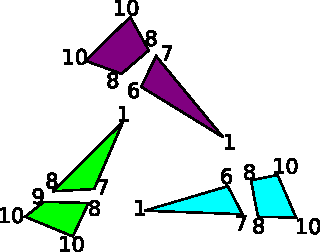
\includegraphics[width = .45\linewidth]{painters.pdf}
			\caption{Mögliche Zerlegung der Dreiecke in Polygone}
			\label{painters}
		\end{figure}
	\end{itemize}
\end{frame}
	
\section{Aufgabe 3}
\begin{frame}
	\frametitle{Aufgabe 3: B\"aume \\Quadtree} 
	\begin{figure}
		\centering
		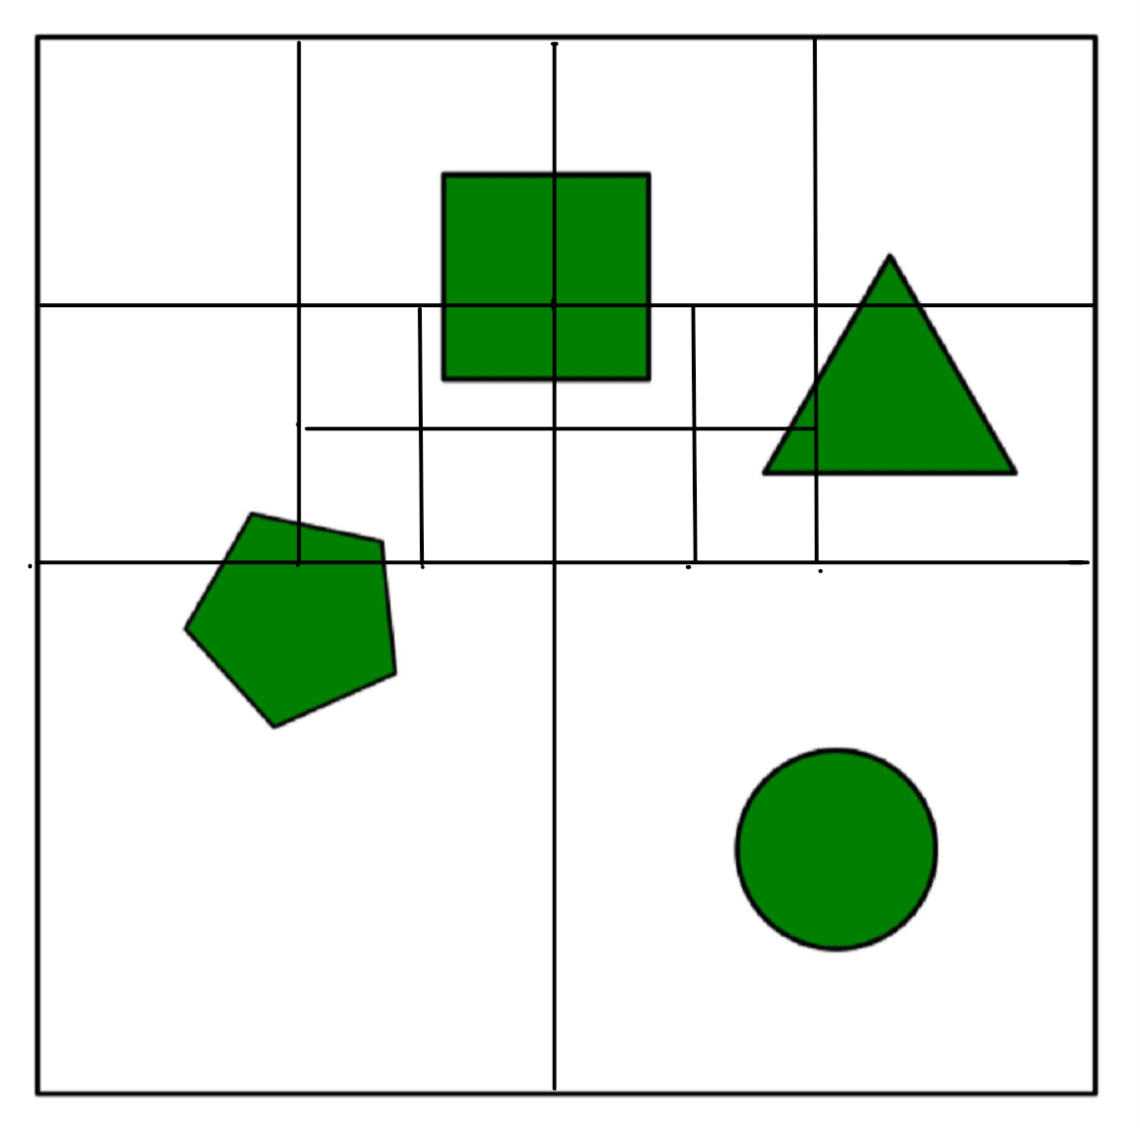
\includegraphics[width=0.5\textwidth]{Quadtree}
	\end{figure}
\end{frame}

\begin{frame}
	\frametitle{Aufgabe 3: B\"aume \\Quadtree}
	\begin{figure}
		\centering
		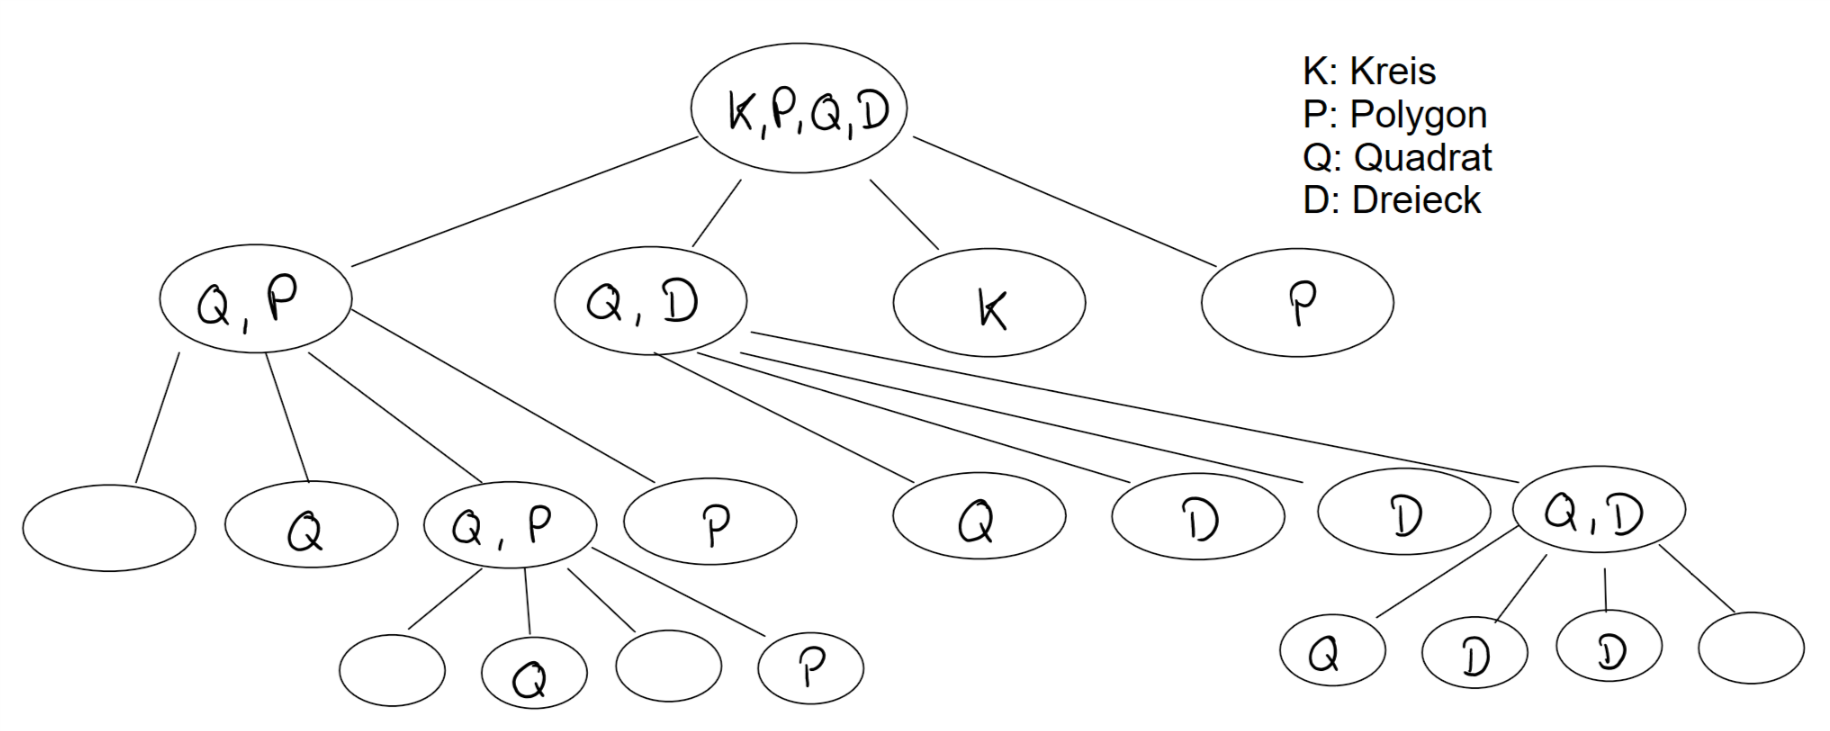
\includegraphics[width=0.9\textwidth]{Quadtree-Nodes}
	\end{figure}
\end{frame}

\begin{frame}
	\frametitle{Aufgabe 3: B\"aume \\BSP} 
	\begin{figure}
		\centering
		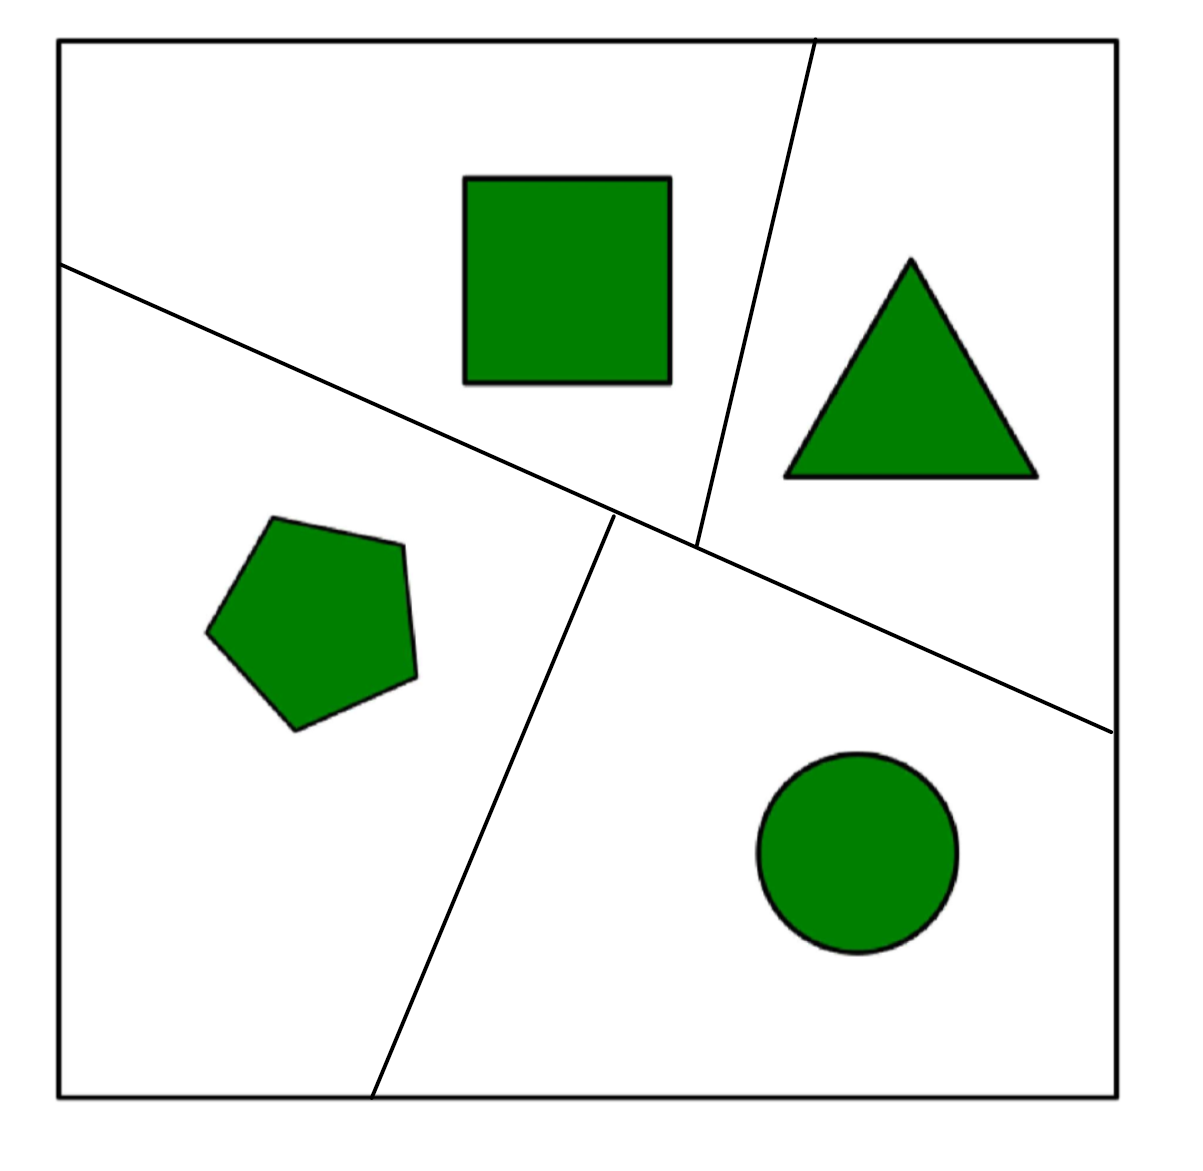
\includegraphics[width=0.5\textwidth]{BSP}
	\end{figure}
\end{frame}

\begin{frame}
	\frametitle{Aufgabe 3: B\"aume \\BSP} 
	\begin{figure}
		\centering
		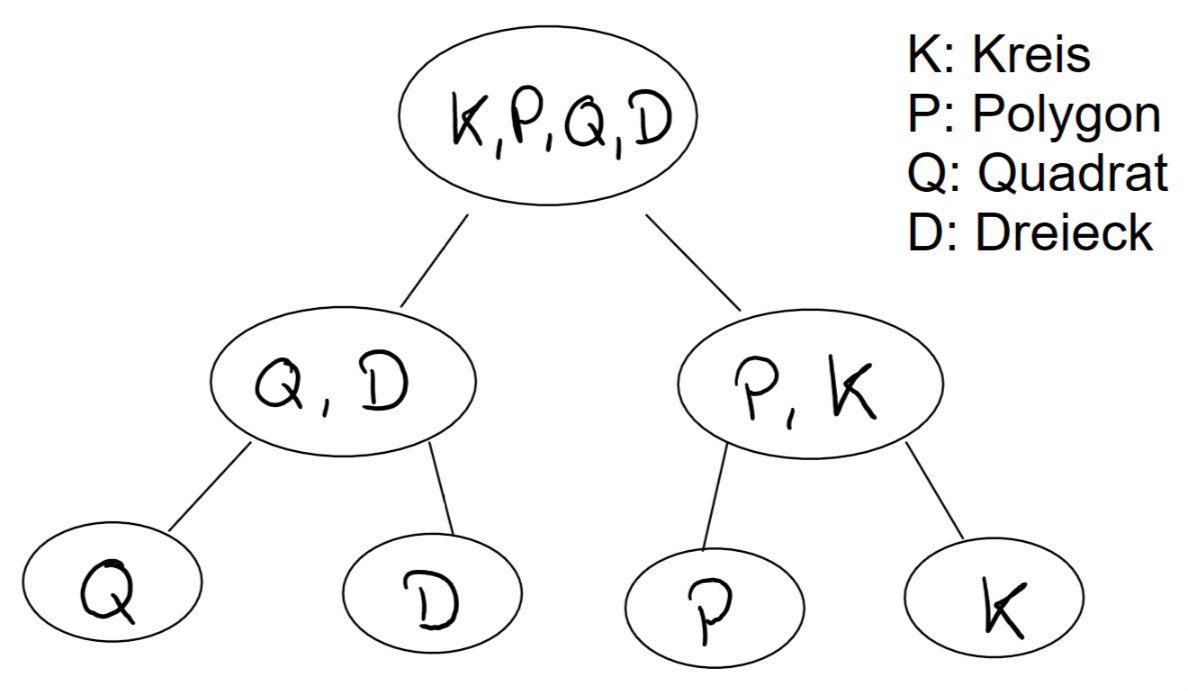
\includegraphics[width=0.8\textwidth]{BSP-Nodes}
	\end{figure}
\end{frame}

\begin{frame}
	\frametitle{Aufgabe 3: B\"aume \\k-d} 
	\begin{figure}
		\centering
		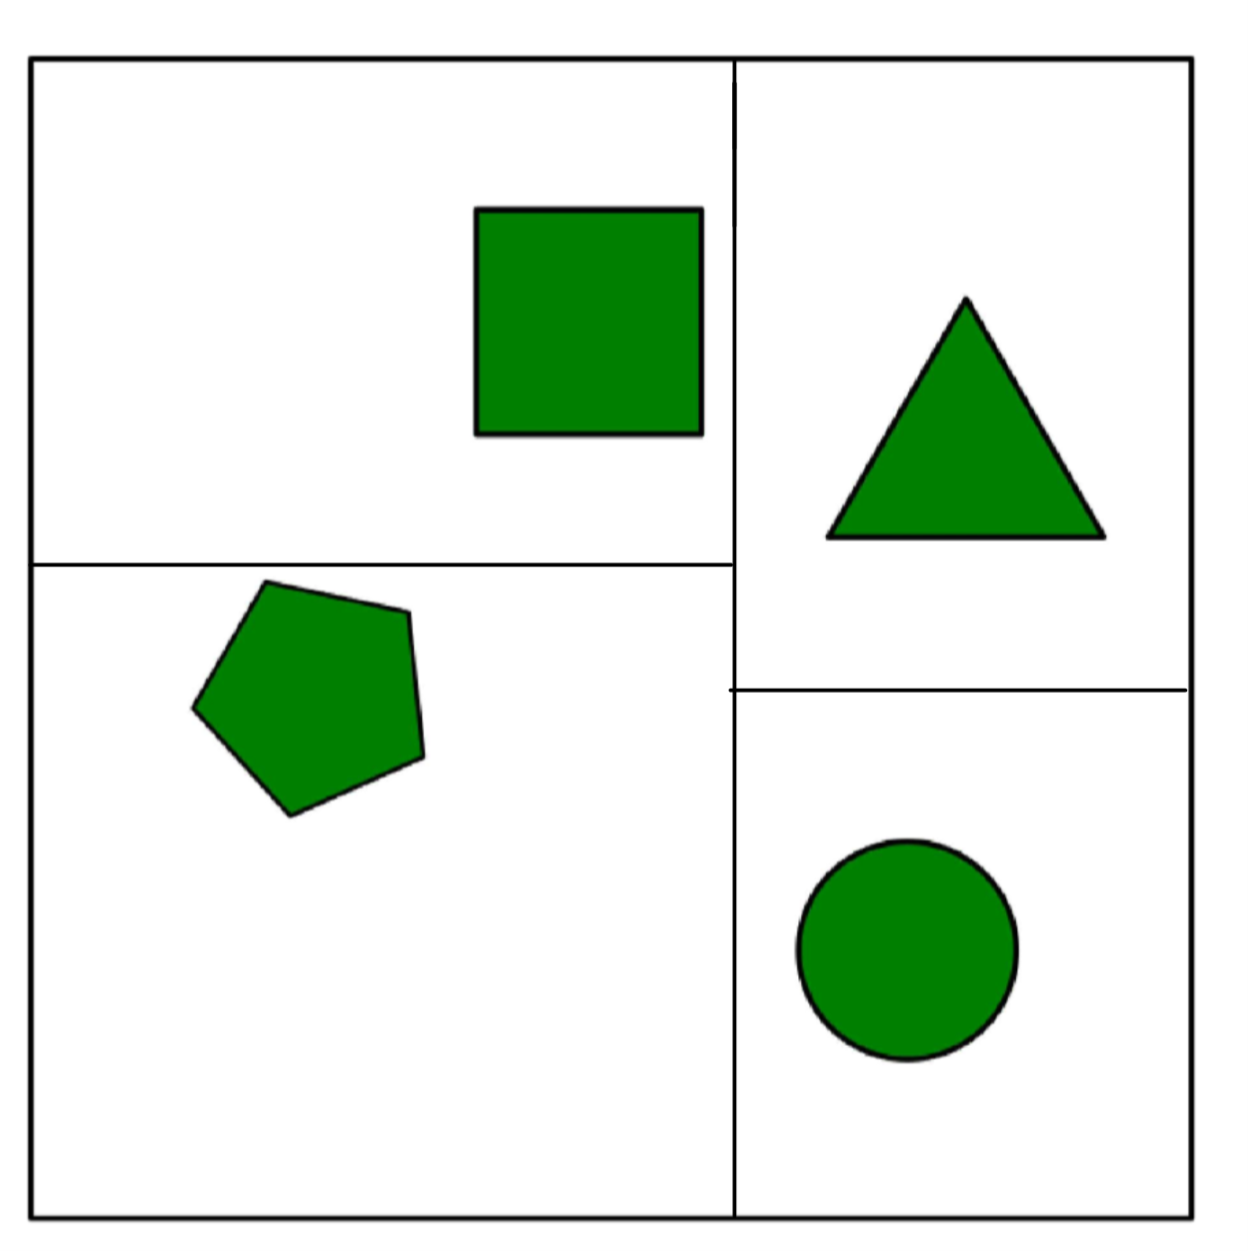
\includegraphics[width=0.5\textwidth]{K-D}
	\end{figure}
\end{frame}

\begin{frame}
	\frametitle{Aufgabe 3: B\"aume \\k-d} 
	\begin{figure}
		\centering
		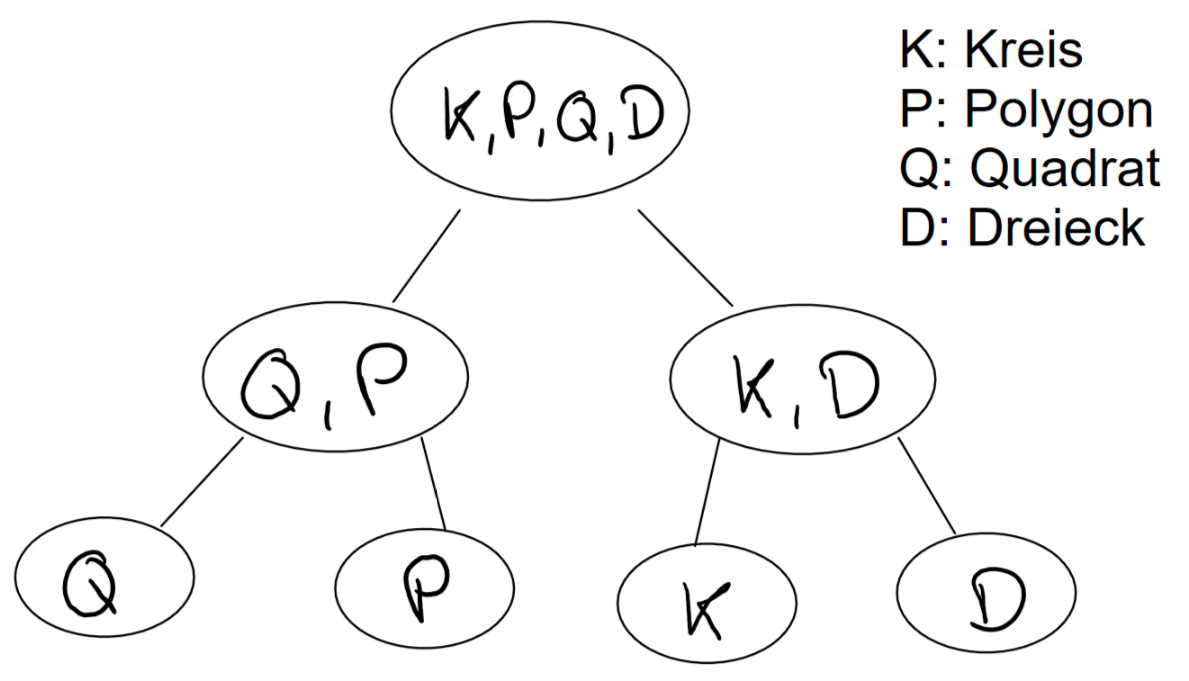
\includegraphics[width=0.8\textwidth]{K-D-Nodes}
	\end{figure}
\end{frame}	

\section{Aufgabe 4}
	\begin{frame}
		\frametitle{Aufgabe 4: Rasterisierung} 
		Die Anwendung des Bresenham-Algorithmusliefert die Werte
		\begin{tabular}{c*{4}{|c}}%>{\tiny}
			\textbf{i} & \textbf{Fehler} & $\textbf{x}_{i}$ & $\textbf{y}_{i}$ & \textbf{neuer\_Fehler} \\
			\hline
			0 & 3.5 & 2 & 2 & 3.5\\
			1 & 3.5 - 4 = -0.5 & 3 & 3 & -0.5 + 7 = 6.5\\
			2 & 6.5 - 4 = 2.5 & 4 & 3 & 2.5\\
			3 & 2.5 - 4 = -1.5 & 5 & 4 & -1.5 + 7 = 5.5\\
			4 & 5.5 - 4 = 1.5 & 6 & 4 & 1.5\\
			5 & 1.5 - 4 = -2.5 & 7 & 5 & -2.5 + 7 = 4.5\\
			6 & 4.5 - 4 = 0.5 & 8 & 5 & 0.5\\
			7 & 0.5 - 4 = -3.5 & 9 & 6 & -3.5 + 7 = 3.5\\
			\hline 
		\end{tabular}. 
	$\vec{x}_{Start} =
	\begin{bmatrix}
	2 \\ 2
	\end{bmatrix}
	 $ und
	 $\vec{x}_{Ziel} =
	 \begin{bmatrix}
	 9 \\ 6
	 \end{bmatrix}
	 $.\\
	{\tiny 
		Mit	$dx=x_{end} - x_{start}$, 
		$dy=y_{end} - y_{start}$ folgt für  $1\leq i \leq x_{end}$ gilt \\		 
		$Fehler_{i}=neuer\_Fehler_{i-1} - dy$, 
		$neuer\_Fehler_{i}=
		\begin{cases}
		Fehler_{i}+dx & \text{,wenn }Fehler_{i} < 0 \\
		Fehler_{i} & \text{,sonst}
		\end{cases}$,\\
		$x_{i}=x_{i-1}$ und 
		$y_{i} = 
		\begin{cases}
		y_{i-1}+1 & \text{,wenn }Fehler_{i} < 0 \\
		y_{i-1} & \text{,sonst}
		\end{cases}$.\\
		Sowie für $i=0$ gelten die Startwerte, sowie $Fehler_{0}=0.5 \cdot dx$.}
	\end{frame}
	\begin{frame}
	\frametitle{Aufgabe 4: Rasterisierung} 
	Damit folgt für die Grafik \\
	\centering
	\begin{tabular}{|*{10}{c|}}
		\hline
		& & & & & & & & & \\ %y=7
		\hline
		& & & & & & & & \cellcolor{black} & \\ %y=6
		\hline
		& & & & & & \cellcolor{black} & \cellcolor{black} & & \\ %y=5
		\hline
		& & & & \cellcolor{black} & \cellcolor{black} & & & & \\ %y=4
		\hline
		& & \cellcolor{black} & \cellcolor{black} & & & & & & \\ %y=3
		\hline
		& \cellcolor{black} & & & & & & & & \\ %y=2
		\hline
		& & & & & & & & & \\ %y=1
		\hline
	\end{tabular}.
	\end{frame}
\end{document}
